\subsection{Development of Self-Adaptive Systems}

For self-adaptive systems (SAS) some activities that traditionally occur at development-time are moved to runtime.  In\cite{andersson_software_2013}
was proposed a process for development of adaptive systems.
Activities performed externally are referred as \emph{off-line activities}, and activities performed internally as \emph{on-line activities}.

The right-hand side of Figure~\ref{fig:sas_lifecycle} depicts a running SAS. At this system we have \emph{Domain Logic} that solves that is responsible for final user goals achievements. And also, \emph{Adaptation Logic}, that is responsible to adapt the system in response to changes in the environment. Adaptation logic implements a control loop in line with the monitor-analyze-plan-execute (MAPE) loop~\cite{kephart_vision_2003}.

The left-hand side of Figure~\ref{fig:sas_lifecycle} represents a staged life-cycle model. Off-line activities work on artifacts such as design model and source code in a product repository and not directly on the running system.


\begin{figure}[!htb]
  \centering
  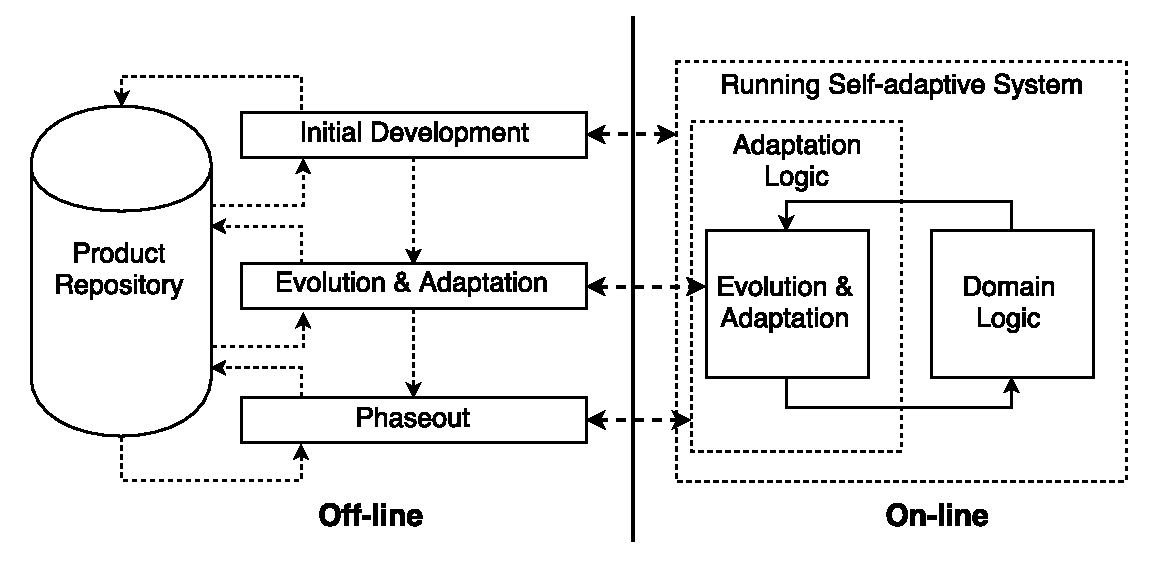
\includegraphics[width=\linewidth]{sas_lifecycle}
  \caption{A Life-cycle model for Self-Adaptation Software System\cite{andersson_software_2013}}
  \label{fig:sas_lifecycle}
\end{figure}
